\documentclass[12pt]{article} % Default font size is 12pt, it can be changed here
\usepackage{geometry} % Required to change the page size to A4
\usepackage{graphicx} % Required for including pictures
\usepackage{float} % Allows putting an [H] in \begin{figure} to specify the exact location of the figure
\usepackage{wrapfig} % Allows in-line images such as the example fish picture
\usepackage{amssymb}
\usepackage{url}
\usepackage{pdfpages}
\geometry{a4paper} % Set the page size to be A4 as opposed to the default US Letter
\graphicspath{{graphs/}{img/}} % Specifies the directory where pictures are stored
\linespread{1.2} % Line spacing

\begin{document}

%----------------------------------------------------------------------------------------
%	TITLE PAGE
%----------------------------------------------------------------------------------------
\begin{titlepage}

\newcommand{\HRule}{\rule{\linewidth}{0.5mm}} % Defines a new command for the horizontal lines, change thickness here

\center % Center everything on the page

\textsc{\LARGE Universit\'a di Trento}\\[0.8cm] % Name of your university/college
\textsc{\Large Corso HCI A.A. 2014-2015}\\[0.8cm] % Major heading such as course name
\textsc{\large Partecipatory Development}\\[1.5cm] % Minor heading such as course title

\HRule \\[0.8cm]
{ \huge \bfseries Gestione delle labels di Github}\\[0.4cm] % Title of your document
\HRule \\[2cm]

\begin{minipage}{0.4\textwidth}
\begin{flushleft} \large
\begin{tabular}{ll}
Bortoli \textsc{Gianluca} & \makebox[2cm][r]{159993} \\
Brugnara \textsc{Martin} & \makebox[2cm][r]{157791} \\
Dellera \textsc{Andrea} & \makebox[2cm][r]{158365} \\
Hoxha \textsc{Fatbardha} & \makebox[2cm][r]{161003}
\end{tabular}
\end{flushleft}
\end{minipage}

\vfill % Fill the rest of the page with whitespace
{\large \today}\\[3cm] % Date, change the \today to a set date if you want to be precise
\end{titlepage}

%----------------------------------------------------------------------------------------
%	TABLE OF CONTENTS
%----------------------------------------------------------------------------------------
\tableofcontents % Include a table of contents

\newpage % Begins the essay on a new page instead of on the same page as the table of contents 

\section{Introduzione}
Il primo obiettivo di questo progetto consiste nell'analizzare \'e quali siano le principali barriere nella partecipazione ai progetti open source, che oggigiorno sono diventati sempre pi\'u numerosi e di una certa rilevanza (addirittura a livello mondiale in alcuni casi).\\
Il nostro interesse \'e ricaduto proprio in queste problematiche che affliggono questo tipo di progetti, dal momento che sono state ravvisate anche in prima persona durante il corso dei nostri studi.\\
Questo approfondimento deriva in parte anche dalla nostra propensione ed interesse per l'utilizzo di software open source durante la nostra carriera universitaria e lavorativa.\\
Lo scopo finale \'e quello di trovare e formulare una possibile soluzione al problema della gestione delle etichette su Github (la piattaforma principe per lo sviluppo open source), dal momento che essa \'e attualmente molto confusionaria e poco ben gestita, soprattutto in progetti di una certa complessit\'a e grandezza.
\newpage

\section{Interviste}
Il primo passo per l'individuazione delle principali problematiche legate all'ambito della partecipazione ai progetti open source \'e stata fatta tramite delle interviste. Questo tipo di ricerca si presta molto alla valutazione di barriere di questo tipo, dal momento che l'intervistato non si sente limitato nell'esprimersi (come potrebbe risultare da un questionario a risposta multipla), ma al contempo non ha la percezione di dilungarsi troppo (come invece potrebbe accadere se viene presentato un questionario a domanda aperta) che potrebbe indurlo a non scrivere tutto ci\'o che pensa.\\
Con il tramite dell'intervista "faccia a faccia" questi inconvenienti vengono meno: la persona si sente pi\'u libera di discutere con l'intervistatore che pone le domande e non blocca l'intervistato mentre sta rispondendo, non interrompendo cos\'i il flusso delle idee (che \'e la parte essenziale e di reale interesse dell'intera intervista).\\
\subsection{Traccia}
La traccia \footnote{\url{http://disi.unitn.it/~deangeli/homepage/lib/exe/fetch.php?media=teaching:hci:hci2014_2015:intervista_pd_motivazioni.pdf}} delle domande da porre all'intervistato ci \'e stata fornita direttamente dalla dottoressa Bordin, poich\`e tale argomento non era ancora stato trattato a lezione nel momento in cui abbiamo svolto questa parte del progetto.\\
Essa prevedeva delle domande mirate principalmente a capire:
\begin{itemize}
\item se e quali software open source vengono utilizzati
\item se l'intervistato partecipi/abbia partecipato attivamente a tali progetti
\item quali siano le motivazioni che lo hanno portato a farlo oppure no
\item cosa significhi \emph{partecipare} ad un progetto open source
\end{itemize}
\subsection{Analisi dei risultati}
%-------
% inserire numeri di intervistati
%-------

Il campione su cui \'e stata effettuata l'intervista non \'e molto eterogeneo (come \'e possibile vedere dalla Figura \ref{fig:distribuzione}, dal momento che \'e stato pi\'u immediato intervistare delle persone all'interno del nostro corso di laurea piuttosto che di altri atenei o dei lavoratori.

\begin{figure}[H] 
\center{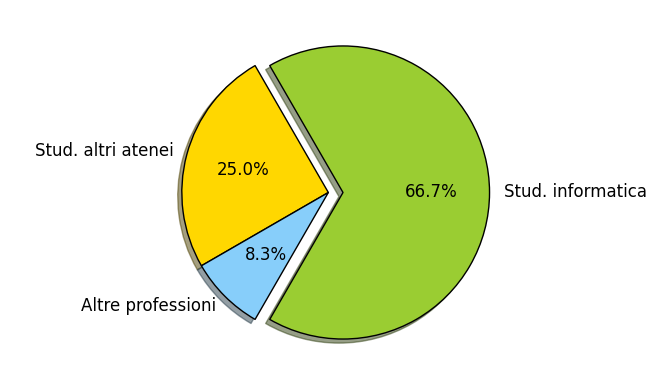
\includegraphics[width=0.8\linewidth]{interviewed_distribution.png}}
\caption{Distribuzione della professione delle persone intervistate.}
\label{fig:distribuzione}
\end{figure}

Abbiamo potuto notare come gli unici due intervistati che hanno contribuito attivamente a progetti open source provenissero esclusivamente da un ambito informatico. Inoltre, all'interno del gruppo stesso ben pochi lo hanno fatto, come \'e possibile notare dalla Figura \ref{fig:distribuzioneInformatica}.\\
Ci\'o ci permette di creare un profilo di utenza specifica (una \emph{personas}) in grado di prendere parte a questa tipologia di progetti. 

\begin{figure}[H] 
\center{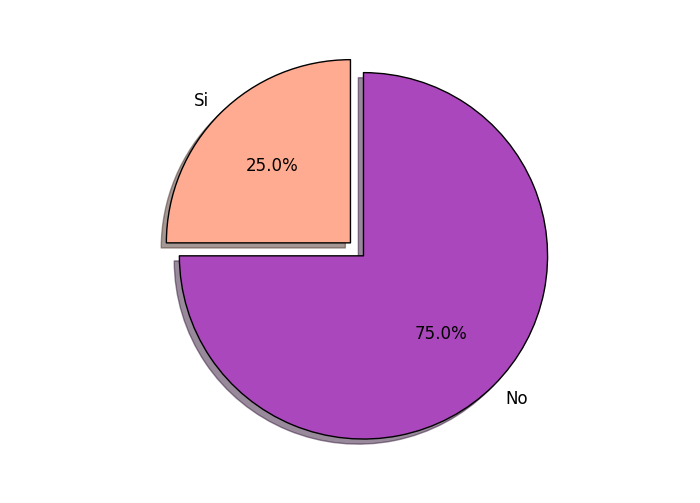
\includegraphics[width=0.8\linewidth]{interviewed_participation.png}}
\caption{Persone che hanno attivamente partecipato a progetti open source tra gli studenti di informatica.}
\label{fig:distribuzioneInformatica}
\end{figure}

Da ci\'o si evince che l'ambito e la possibilit\'a di parteciparvi \'e molto ristretto e ci\'o ci permette di delineare una \emph{personas} con delle caratteristiche ben definite, quali:
\begin{itemize}
\item consistente background informatico
\item interesse verso il campo specifico del progetto considerato
\item tempo e impegno da dedicarvi
\end{itemize}

In aggiunta abbiamo notato come lo \emph{scenario} accademico incentivi e contribuisca ad utilizzare specifici software open source e, di conseguenza, aumenti la probabilit\'a che uno studente si interessi e ne possa far parte. 
%-------
% descrizione di cosa sia una personas?
%-------
\newpage

\section{Benchmarking}
Durante questa fase abbiamo scelto di concentrarci su tre progetti open source: NeoVim, CyanogenMod e OpenOffice.\\
Dopo averli presentati e descritti durante un workshop, abbiamo analizzato i pro ed i contro di ciascuno, da cui \'e emerso che molti utenti utilizzano spesso questi software sia in ambito personale che lavorativo.\\
Quelli da noi considerati sono gratuiti \footnote{Non bisogna confondere il concetto di open source con quello di freeware: che un software sia open source non implica necessariamente che sia anche distribuito gratuitamente (ad esempio RedHat)}, di facile utilizzo e mantenuti costantemente aggiornati dalla comunit\'a di sviluppo. In pi\'u le funzionalit\'a offerte sono molto simili a quelle dei rispettivi software equivalenti, se non addirittura le medesime.\\
Al contrario, essi non vengono largamente utilizzati a causa della scarsa conoscenza del prodotto, dal momento che vengono scarsamente pubblicizzati soprattutto a livello delle istituzioni pubbliche, e per la loro usabilit\'a sulla quale spesso non viene fatto uno studio molto approfondito.\\
\subsection{Contribuire ad un progetto}
Dalle interviste \'e emerso che il significato dato al termine \emph{contribuire} \'e quello di mettere a disposizione le proprie competenze per il miglioramento di un software e/o la risoluzione di eventuali problemi ad esso legati.\\
Le motivazioni che spingono a contribuire sono molte: dalla semplice soddisfazione per aver risolto un bug, all'arricchimento personale e l'esperienza acquisita che ne consegue, passando per la necessit\'a di dover implementare una funzionalit\'a che risolva un problema che si ha nel proprio lavoro.\\
Al contrario, altrettanti sono i motivi che spingono le persone a non contribuire, tra i quali la mancanza di tempo e di competenze e soprattutto la qualit\'a e disponibilit\'a di informazioni riguardanti un progetto specifico. Quest'ultimo a nostro avviso risulta essere il pi\'u rilevante, dal momento che un utente (con magari delle capacit\'a per farlo) si trova a non poter contribuire a causa della mancanza di linee guida su come si possa farlo.		 Ci\'o potrebbe sembrare banale a primo impatto, ma \'e una costante in tutti i progetti da noi presi in considerazione.
\newpage

\section{Design library: NeoVim}
Nella nostra \emph{design library} ci siamo concentrati sul progetto di NeoVim per poter individuare sia degli esempi di cattiva e che di buona progettazione da cui prendere spunto.\\
\subsection{Buoni esempi}
Facciamo ora una lista degli esempi più significativi di un design pensato e studiato appositamente per far s\iì che l'utente interessato a partecipare riesca a farlo nel modo migliore possibile.\\
Abbiamo notato come sia il sito di NeoVim che la gestione della codebase su Github siano state progettate secondo il paradigma dell'\emph{user driven design}, il quale mira massimizzare l'usabilit\'a del prodotto.

\begin{figure}[H] 
\center{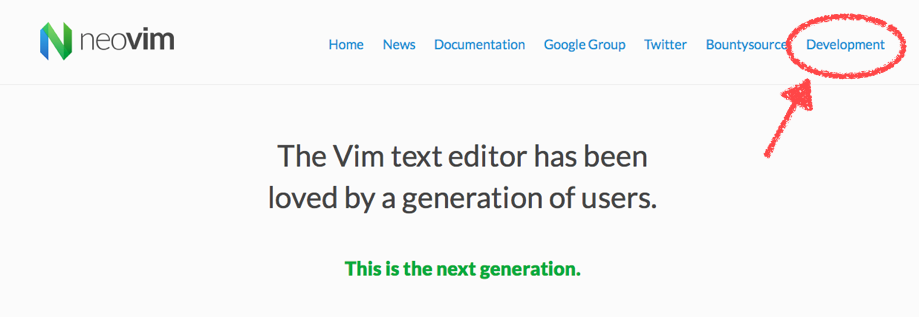
\includegraphics[width=0.8\linewidth]{buonesempio1.png}}
\caption{Homepage di NeoVim.}
\label{fig:buonesempio1}
\end{figure}

Dalla Figura \ref{fig:buonesempio1} si pu\'o notare come il gruppo di sviluppo del progetto preso in considerazione indichi chiaramente nella pagina principale una sezione per chi volesse contribuire. Gi\'a da questo possiamo capire come si punti sullo sviluppo di terze persone: per questo motivo il link al codice sorgente del software su Github viene messo nel menu principale, in modo che sia di facile reperibilit\'a.

\begin{figure}[H] 
\center{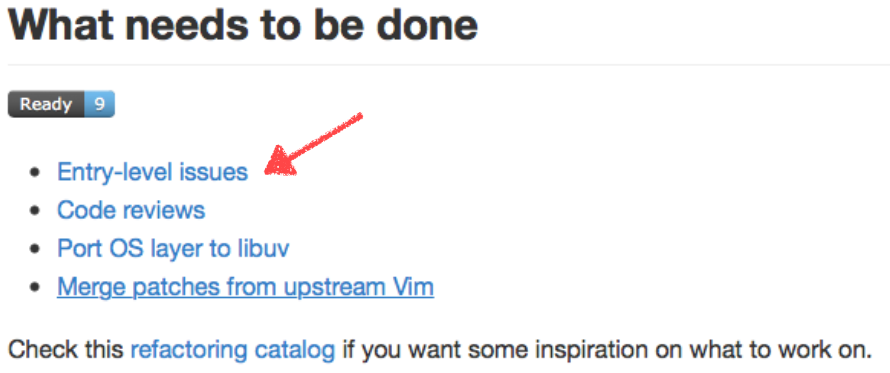
\includegraphics[width=0.65\linewidth]{buonesempio2.png}}
\caption{Cosa c'\'e da fare.}
\label{fig:buonesempio2}
\end{figure}

Un altro dei problemi riscontrati durante la fase di benchmarking \'e quello di non ritenere le proprie capacit\'a sufficienti per dare il proprio contributo. Ci\'o \'e stato parzialmente risolto (Figura \ref{fig:buonesempio2}) introducendo dei \emph{livelli di difficolt\'a} per le issues/bug presenti nel software.\\
\'E stato introdotta un'etichetta per i problemi di pi\'u facile risoluzione (entry level), cosa che non avevamo notato in qualsiasi altro progetto da noi preso in considerazione.

\begin{figure}[H] 
\center{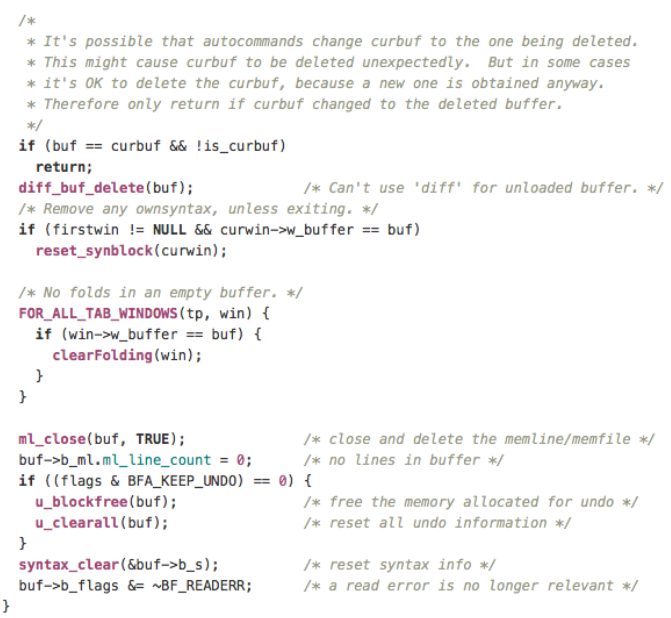
\includegraphics[width=0.65\linewidth]{buonesempio3.png}}
\caption{Homepage di NeoVim.}
\label{fig:buonesempio3}
\end{figure}

Infine, viene posta molta cura nella documentazione e nei commenti all'interno del codice. Ci\'o aiuta chi interviene in quella porzione di sorgente per poter capire meglio e senza eccessiva difficolt\'a cosa faccia una certa porzione di codice.\\
Inoltre, alla nascita di NeoVim sono state decise delle linee guida ben precise su come si dovesse indentare/organizzare il codice e soprattutto su come commentarlo, in modo da non creare disomogeneit\'a all'interno del progetto (il che creerebbe non pochi problemi di comprensione).

\subsection{Cattivi esempi}
Al contrario, abbiamo individuato delle parti che risultavano di difficile comprensione e che potevano creare dei problemi con chi volesse interagire.

\begin{figure}[H] 
\center{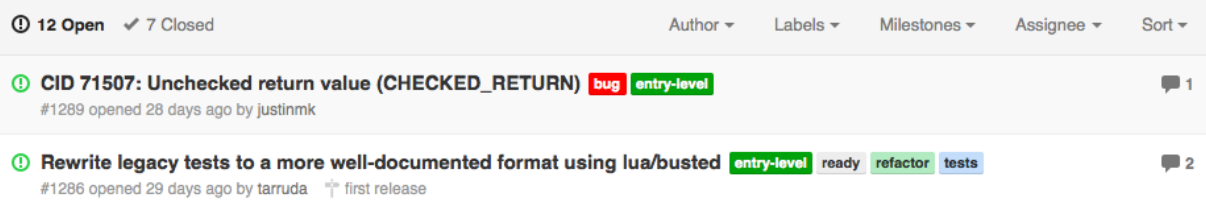
\includegraphics[width=0.65\linewidth]{cattivoesempio1.png}}
\caption{Etichette assegnate alle issue su Github.}
\label{fig:cattivoesempio1}
\end{figure}

Dalla Figura \ref{fig:cattivoesempio1} già ad un primo impatto si può notare come le etichette assegnate alle issue ancora da risolvere siano poco esplicative e, a volte, ridondanti.\\
Questo crea molta confusione nel momento in cui lo sviluppatore che vuole dare il proprio contributo controlla cosa ci sia da fare e/o correggere, trovandosi davanti una miriade di labels con i colori più disparati e visualizzate in modo disorganizzato e con poca coerenza.

\begin{figure}[H] 
\center{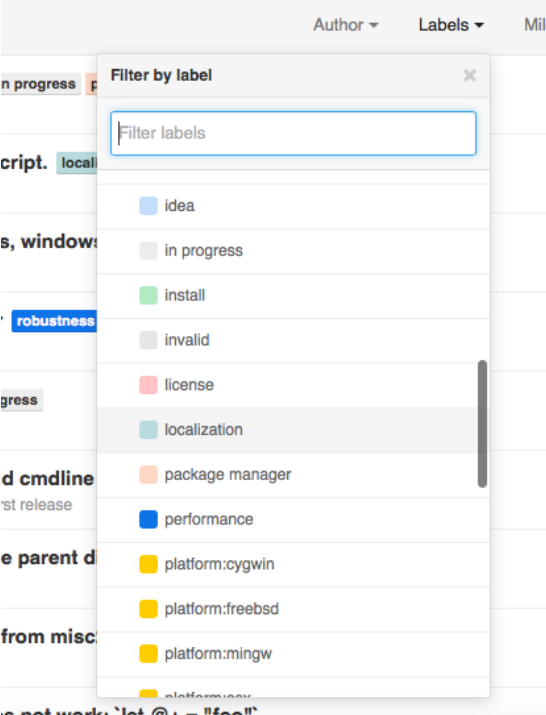
\includegraphics[width=0.4\linewidth]{cattivoesempio2.png}}
\caption{Menu per la selezione delle labels.}
\label{fig:cattivoesempio2}
\end{figure}

Quello della coerenza e dei colori diventa ancora di più un problema nel momento in cui si vuole filtrare tutte le issue per labels.\\
A colori molto simili, talvolta identici tra loro, sono associate delle problematiche e delle aree di lavoro molto differenti tra loro. Come si pu\`o vedere dalla Figura \ref{fig:cattivoesempio2}, le voci \emph{licence} e \emph{package manager} hanno una colorazione quasi indistinguibile, nonostante riguardino due ambiti molto diversi.

\begin{figure}[H] 
\center{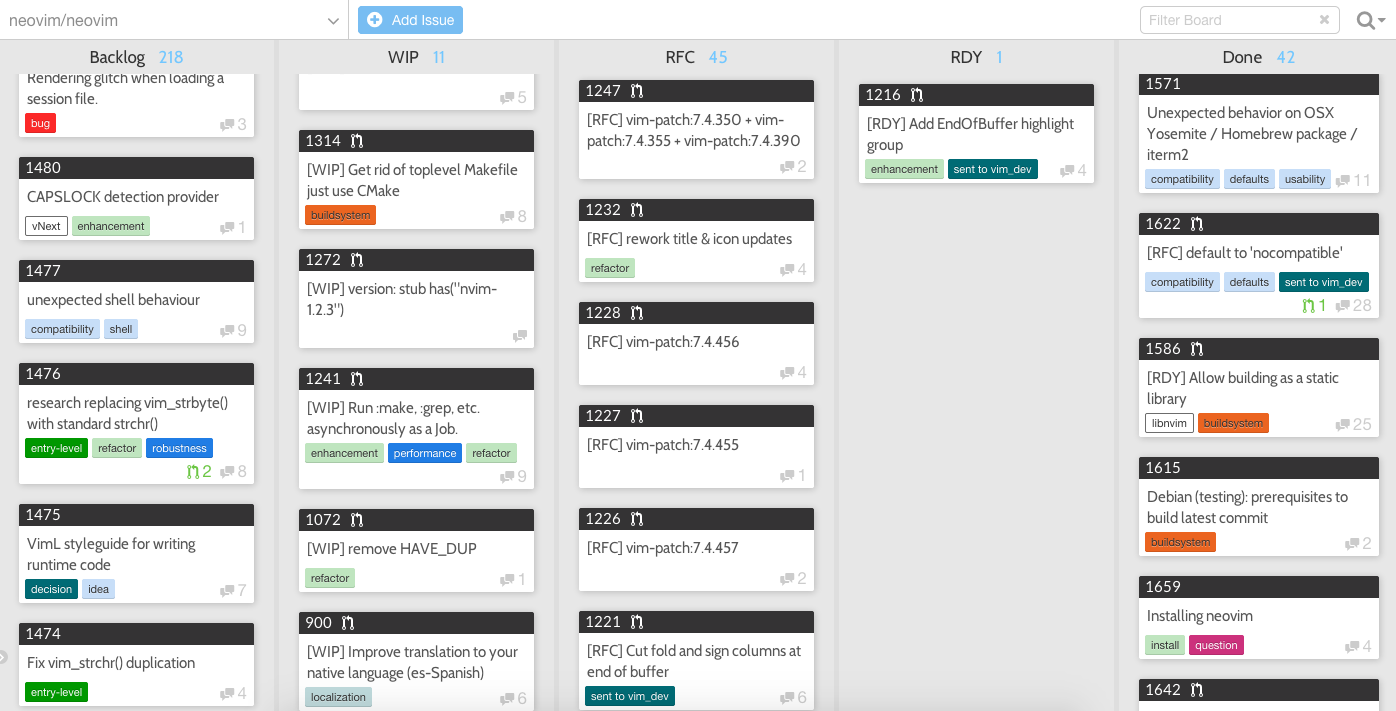
\includegraphics[width=0.8\linewidth]{cattivoesempio3.png}}
\caption{Homepage di NeoVim.}
\label{fig:cattivoesempio3}
\end{figure}

Il problema si estende anche a \emph{Waffle} \footnote{\url{www.waffle.io}}, un tool che permette di gestire in modo pi\`u comodo ed immediato le issues di Github in tempo reale. Grazie a questo software direttamente collegato a Github non c'è la necessit\`a di controllare manualmente lo stato del lavoro, bensì il flusso del lavoro viene direttamente organizzato in base ai commit e alle issue a cui fanno riferimento.\\
Dalla Figura \ref{fig:cattivoesempio3} si evince che la visualizzazione del flusso di lavoro viene intaccato e reso di più difficile comprensione a causa della cattiva gestione delle labels. 
\newpage

\section{Prototipi}
Considerando gli esempi raccolti nella design library, avendo visionato i risultati ottenuti dalle interviste e dopo aver identificato quali siano le problematiche che ostacolano maggiormente la partecipazione, abbiamo deciso di porre particolare attenzione alla gestione delle labels su Github.\\
Il lavoro da noi svolto ha come punto di riferimento ci\`o che abbiamo potuto osservare all'interno del progetto di NeoVim.
\subsection{Prototipo a bassa fedelt\'a}
Utilizzando \emph{Balsamiq \footnote{\url{www.balsamiq.com}}} abbiamo realizzato un primo prototipo a bassa fedelt\`a.\\
Le label che fanno riferimento a problemi della stessa area vengono raggruppate in una singola macro-label, espandibile con un click. L'idea \'e quella di implementare il \emph{design pattern} file-cartella.\\ 
Dopo averci riflettuto a fondo, abbiamo deciso di fermarci ad un solo livello di profondit\`a raggiungibile dalla struttura gerarchica delle labels. Ci\'o significa che se un'etichetta appartiene gi\`a ad una macro-label, essa non pu\'o avere ulteriori sotto-label che creino un altro sottoalbero.\\
Questa decisione, per quanto inizialmente potesse sembrare una limitazione nei confronti dell'utente finale, aiuta a mantenere la semplicit\'a e la praticit\'a delle label senza introdurre difficolt\`a di utilizzo.

\begin{figure}[H] 
\center{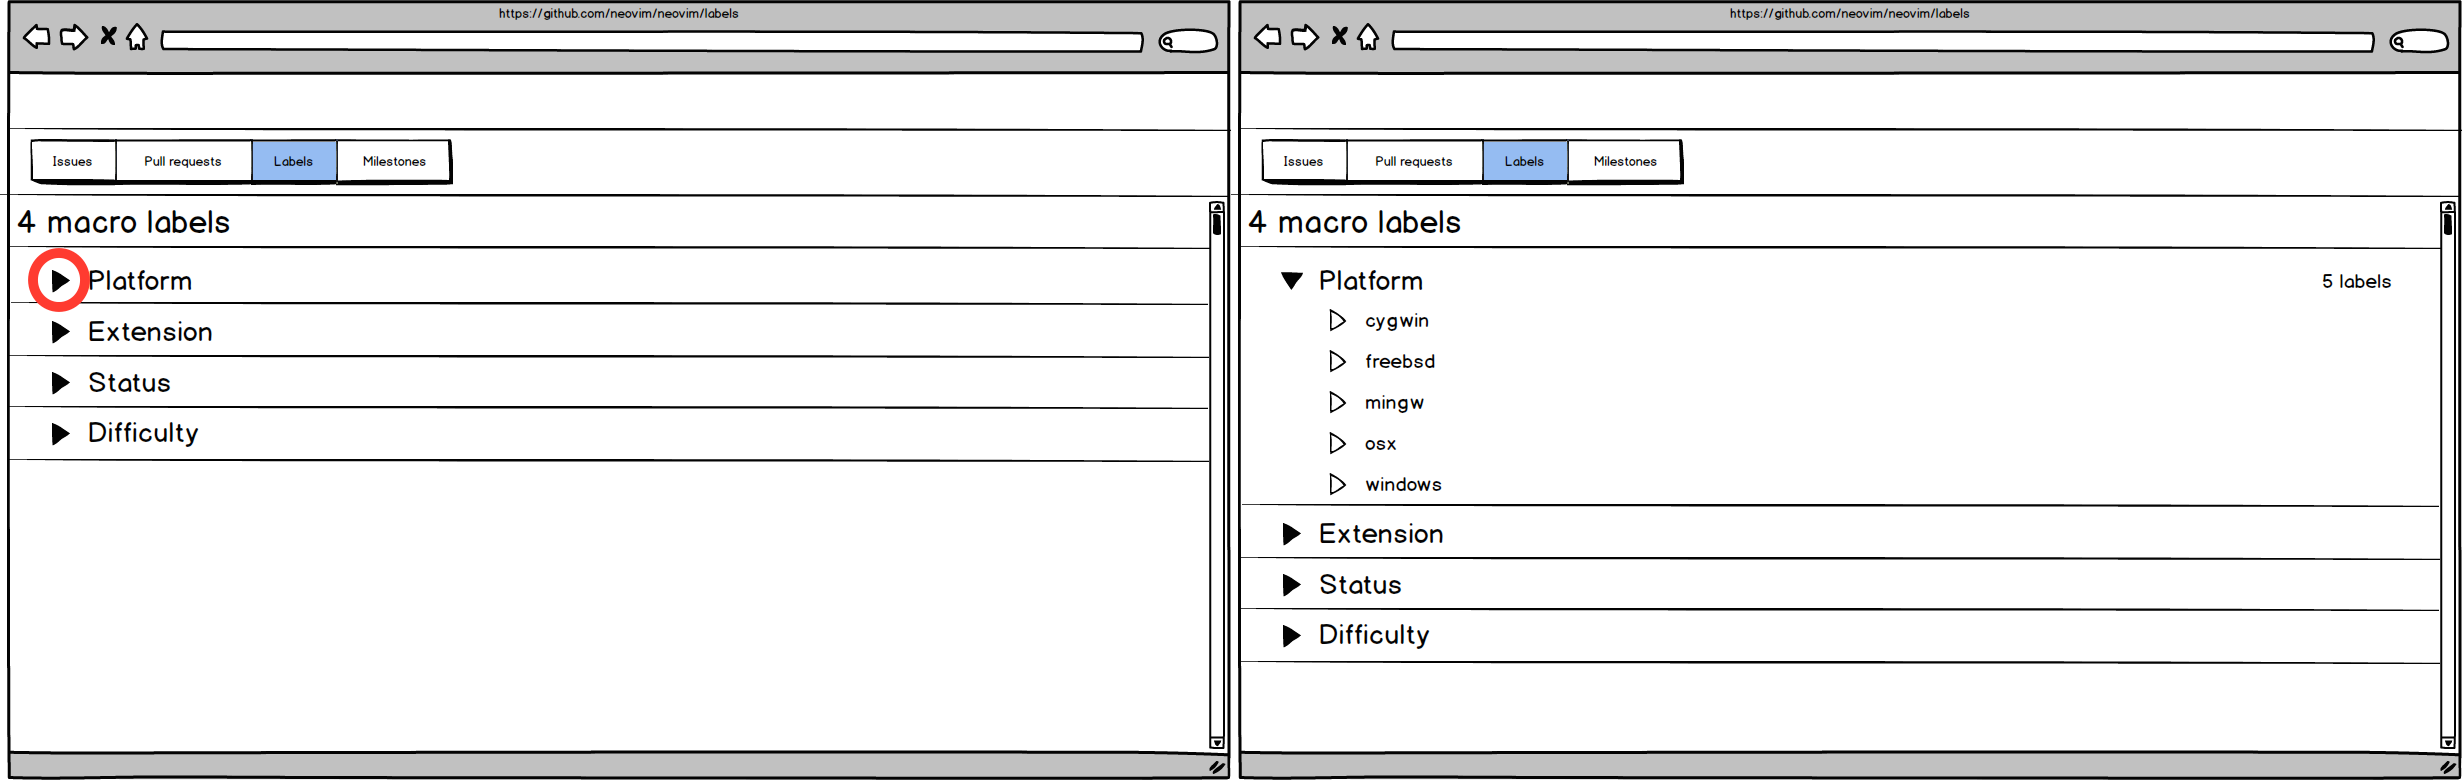
\includegraphics[width=0.9\linewidth]{low_prototype.png}}
\caption{Espansione di una macroarea.}
\label{fig:low_prototype}
\end{figure}

\subsubsection{Decisioni di design}
Dopo aver discusso durante l'ultimo workshop con componenti di altri gruppi e aver ricevuto dei feedback sul nostro prototipo iniziale, abbiamo deciso di seguire la linea iniziale e apportando le seguenti leggere modifiche:
\begin{itemize}
\item un \textbf{triangolo pieno} indica una macro-area che \'e possibile espandere (ovvero che contiene ulteriori labels).
\item un \textbf{triangolo vuoto} indica una macro-area che \emph{non} contiene nulla al suo interno; questo concetto pu\`o ripetersi sia a livello di macro-area che a quello di labels all'interno di una categoria pi\`u grande (Figura \ref{fig:low_prototype}).
\item la scelta di una struttura \textbf{gerarchica} \'e nata dal fatto che chiunque abbia usato prima un gestore di file su un computer ha chiaro l'idea di cartella, tramite la quale \'e possibile organizzare i propri dati in modo coerente. Questo ci permette di utilizzare un concetto non nuovo in un contesto diverso dal 	quale l'utente si aspetta di trovarlo, rendendo l'utilizzo della nostra funzionalit\`a ragionevolmente immediato.
\end{itemize}

\begin{figure}[H] 
\center{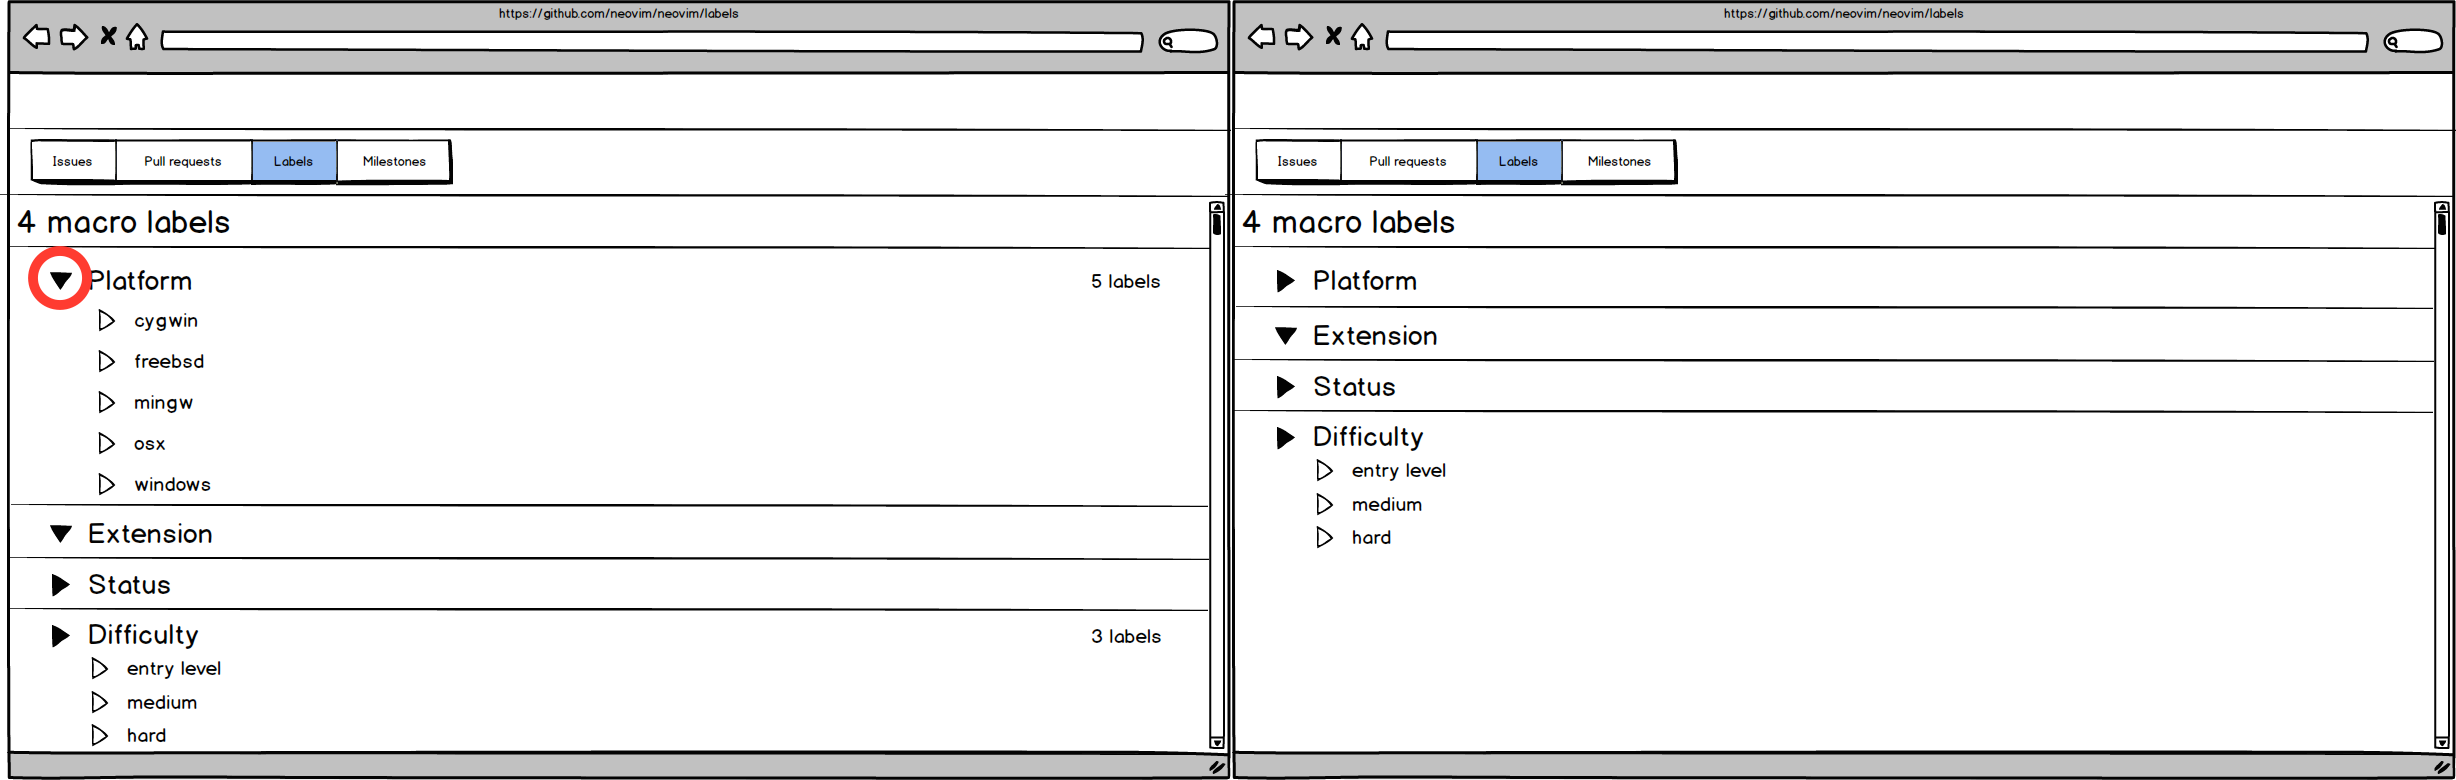
\includegraphics[width=0.9\linewidth]{low_prototype2.png}}
\caption{Struttura gerarchica delle etichette.}
\label{fig:low_prototype2}
\end{figure}

Dalla Figura \ref{fig:low_prototype2} \'e possibile vedere come abbiamo realizzato il nostro prototipo a bassa fedelt\`a conclusivo.

\subsection{Prototipo ad alta fedelt\'a}

\subsubsection{Analisi dei colori}
Dopo aver utilizzato una struttura gerarchica per una visualizzazione più chiara ed intuitiva, abbiamo deciso di soffermarci anche sulla scelta dei \emph{colori} da assegnare alle etichette.\\
Ogni colore, che sia primario oppure secondario, viene percepito da ogni utente in modo diverso e personale: esso è fortemente legato alla sua esperienza e alla sua cultura.\\
Ad esempio, il colore \emph{rosso} nella cultura occidentale viene immediatamente e quasi inconsciamente associato ad un segnale di pericolo o ad un avvertimento che deve catturare l'attenzione. Nella cultura orientale, invece, simboleggia aspetti positivi della vita, come la fortuna e la gioia. Possiamo quindi capire come l'associazione colore-esperienza associata sia estremamente diversa in presenza di contesti sociali differenti.\\

%Cose da dire: generale significato dei colori -> quali colori sono più adatti ad una certa tipologia di label.\\
%colori sono una cosa soggettiva-> per questo motivo l'utente può scegliersi il proprio pattern di colori %togliendo la "limitazione " sulla scelta dei colori l'utente è libero di esprimersi, ma allo stesso tempo può %combinare casini, ad esempio assegnando colori troppo simili fra loro ma questa è una responsabilità che lasciamo all'utente.

% debug
\cite{*}

\newpage
\bibliographystyle{unsrt}
\bibliography{consegna_finale}

\end{document}

%----------------
% miglioramenti: 
%				campione pi\'u eterogeneo e pi\'u vasto per le interviste
%---------------

